\chapter{Diseño y desarrollo\label{sec:disenhoYDesarrollo}}

\textbf{Rápida intro.}

TODO: Demostrar todo el dominio que pueda sobre cuestiones de la carrera.

\section{Diseño}

A la hora de crear un sistema adaptativo como el propuesto, es habitual enfocar el diseño siguiendo el patrón de la figura \ref{fig:diagrama_disenno}

\begin{figure}[htp!]
	\centering
	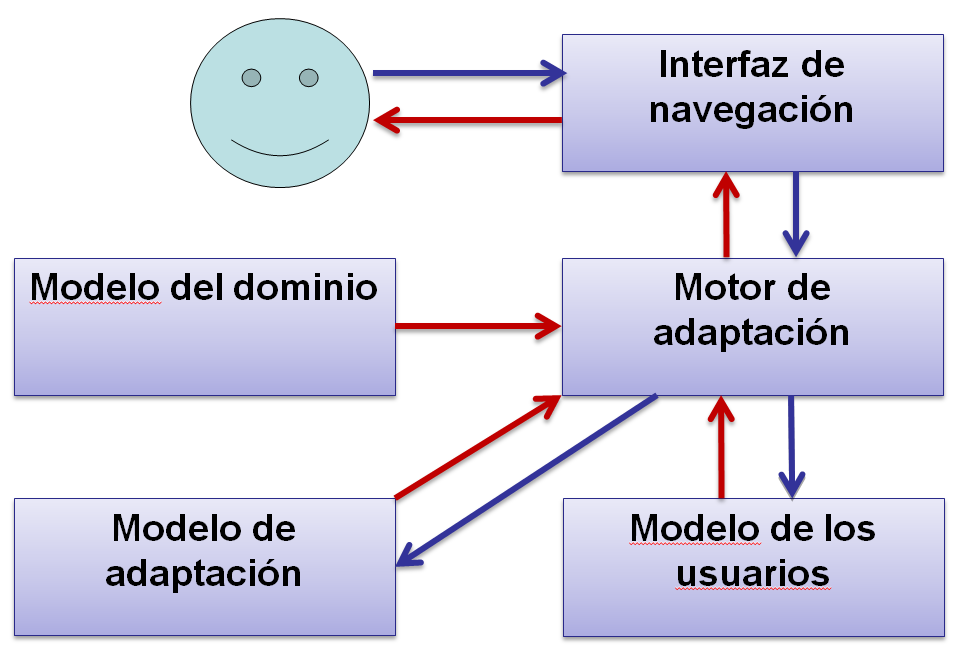
\includegraphics[width=0.75\textwidth,clip=true]{diagrama_disenno}
	\caption{}
	\label{fig:diagrama_disenno}
\end{figure} 

\subsection{Análisis funcional}

\textbf{¿Detallar un análisis funcional? Sí}

\subsection{Modelo del dominio}

\textbf{Estructura de la BD}

\subsection{Modelo de adaptación}

\textbf{Exámenes con distintos niveles}

\subsection{Modelo de usuario}

\textbf{Profesor y alumno}

\subsection{Motor de adaptación}

\textbf{Rápidas notas sobre la aplicación en sí. O no.}

\section{e-valUAM}
